%!TEX root = ../Final_Assignment_SP_ML4IM_2023.tex
\chapter{Results}
\label{ch:results}

% ausführlich
% NOT FINAL - unsure about section structure and names
% alle

This chapter presents the results of the project. This is done by visualising and comparing the results of the different data pre-processing approaches.

% RGB
First af all the results of the default RGB training are presented. The default RGB training was done using the raw RGB data without any preprocessing. The results of this training are shown in Table~\ref{fig:results_rgb}.

% results of rgb
The important values to look at are the precision and recall value of the epochs of the model. The precision and recall values should be as high as possible. The precision value shows the accuracy of detected objects and the recall value shows how many of the actual values were predicted correctly. Normally the two values are getting better with more epochs processed \citep{ultralyticsYOLOPerformance}. But in Figure \ref{fig:results_rgb} the precision is getting lower with each new epoch besides one spike and the recall value stays quite low with one low point.
The box\_loss is also an interesting value to look at. It shows the loss of the bounding boxes. The lower the value the better the bounding boxes are predicted. The box\_loss is getting lower with each epoch which is at first sight a good sign. But in the box loss of the validation it varies a lot. So this model is quite bad at detecting the insects in the RGB data.

\begin{figure}[htbp] 
    \centering
    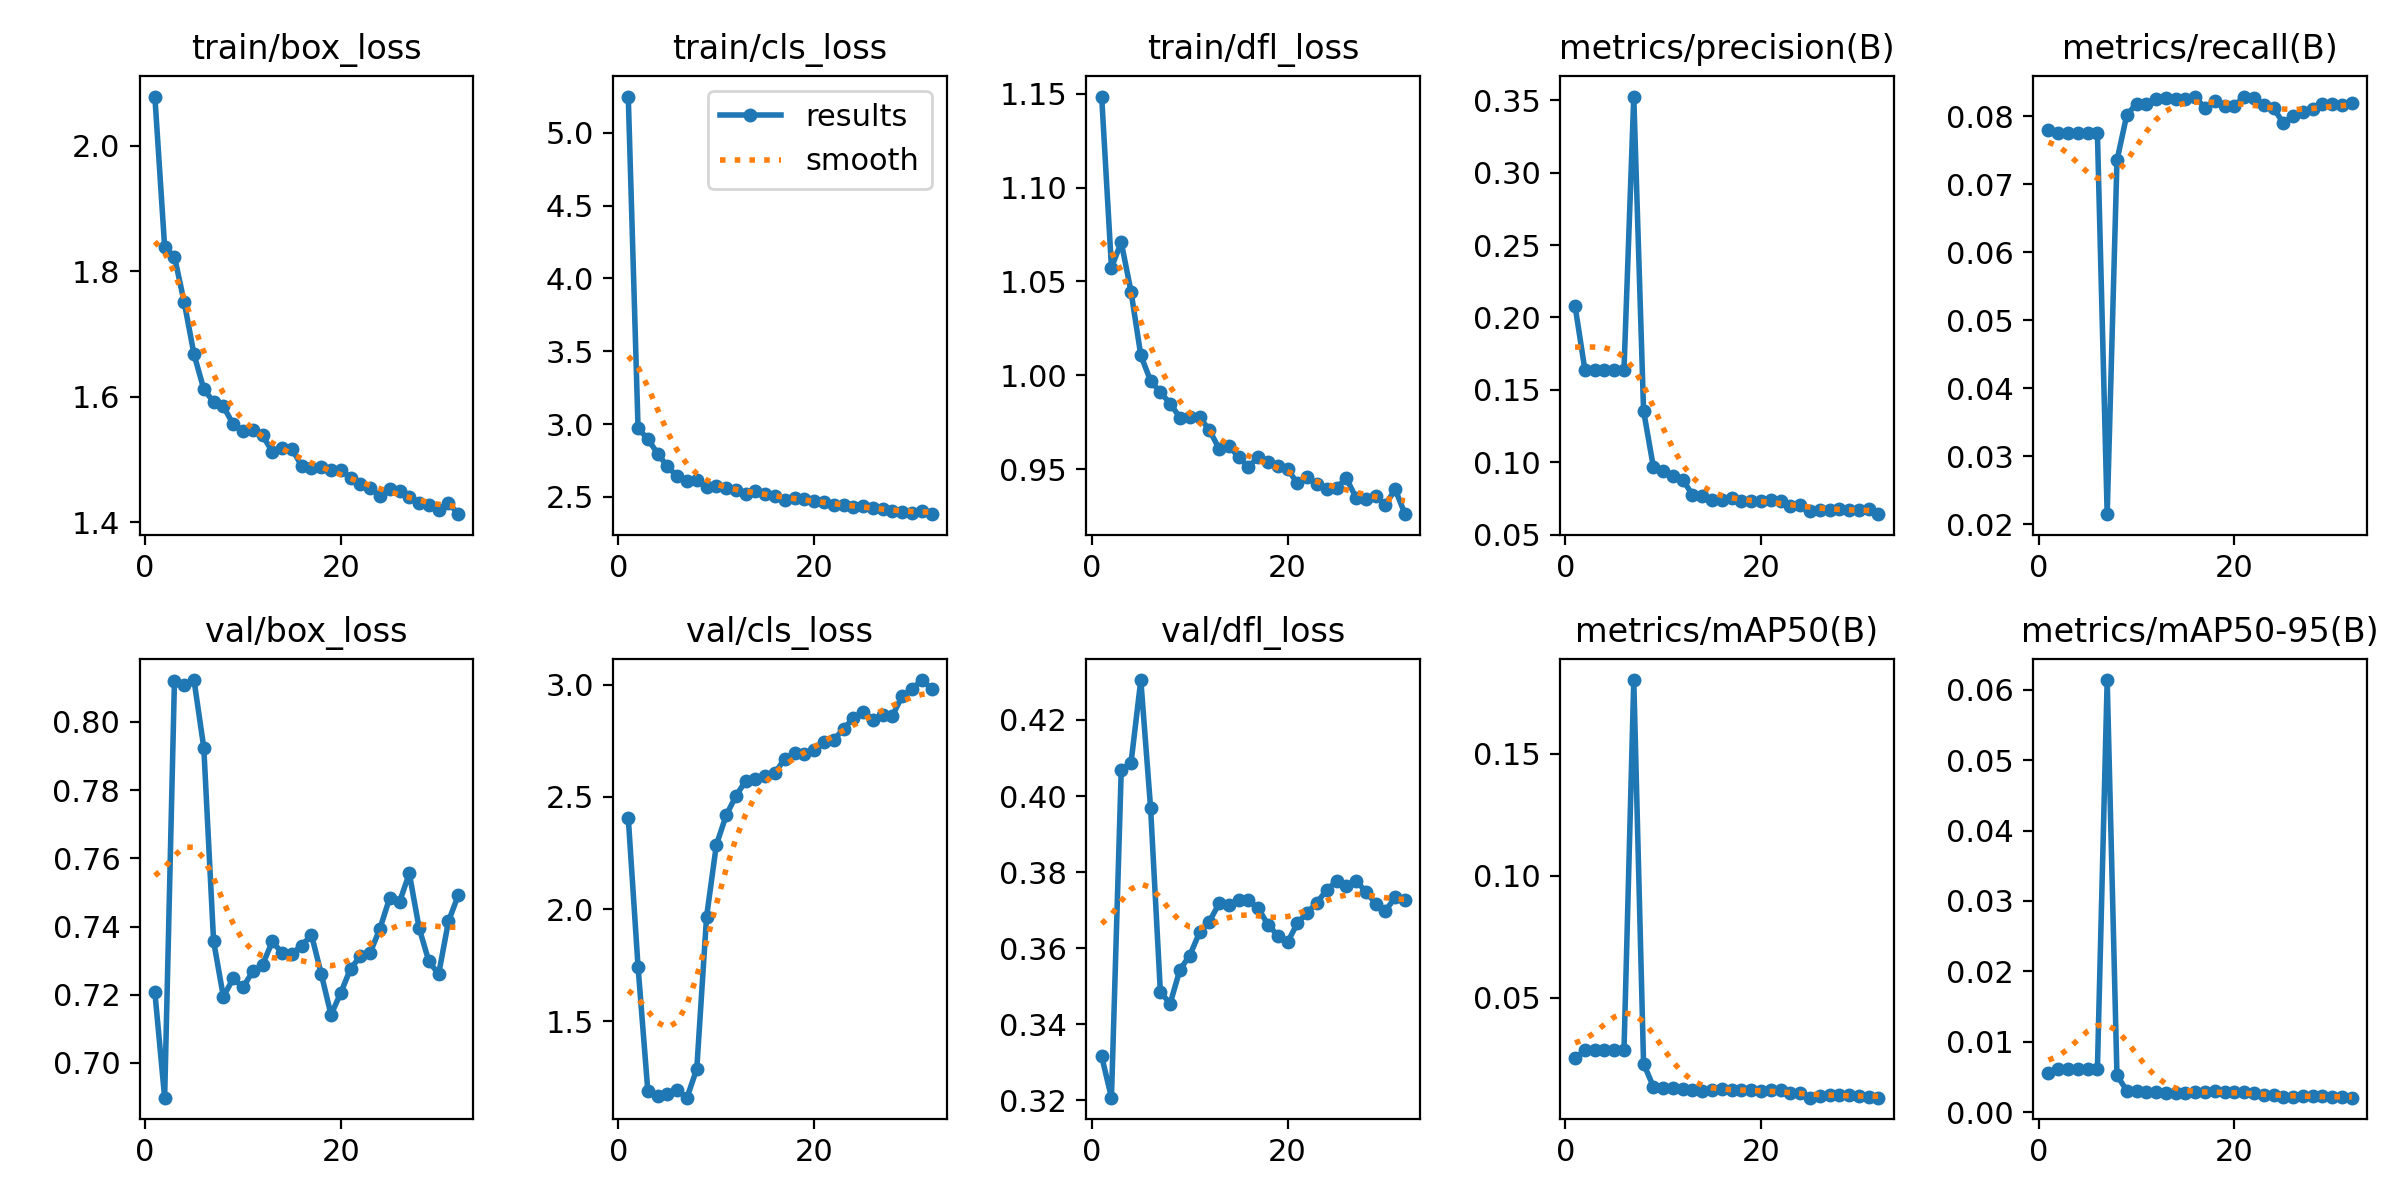
\includegraphics[width=0.8\textwidth]{images/results/rgb_results.png}
    \caption{Results of the model training with RGB data}
    \label{fig:results_rgb}
\end{figure}

% background subtraction

The background subtraction method was then used on the rgb data. The results of this training are shown in Table~\ref{fig:results_bgsub}.

\begin{figure}[htbp] 
    \centering
    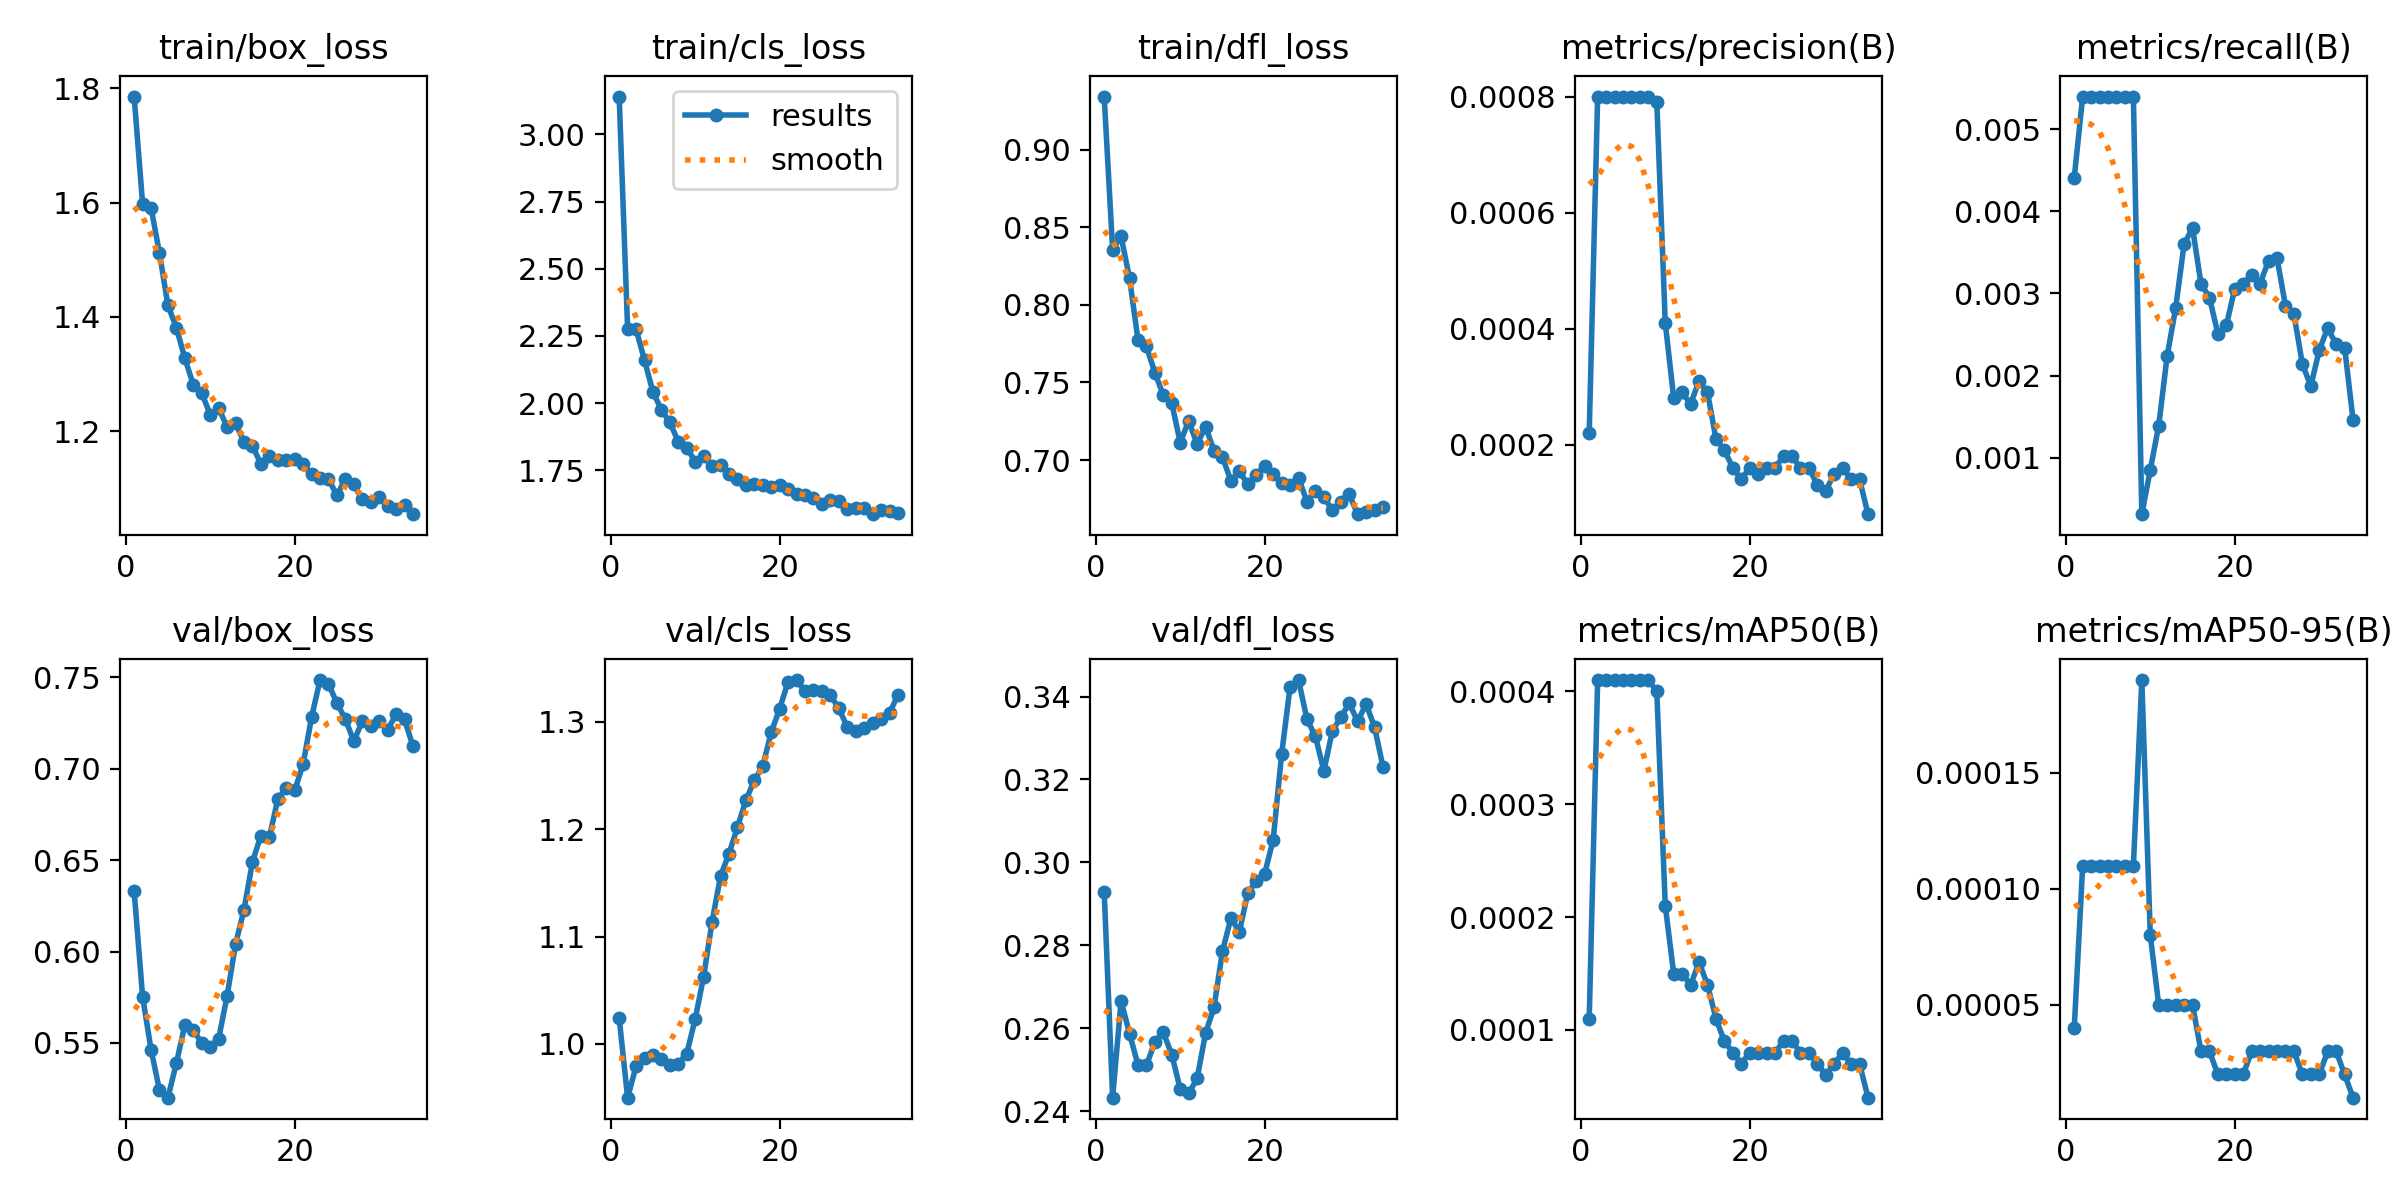
\includegraphics[width=0.8\textwidth]{images/results/bgsub_results.png}
    \caption{Results of the model training with background subtraction}
    \label{fig:results_bgsub}
\end{figure}

% results of background subtraction
The background subtraction model has much lower precision and recall values than the RGB model. At the final epochs it even goes down to lower than 0.0002 but for that the box\_loss looks normal. All in all the the results of the background subtraction model is not good and should normally be better than the RGB model.

% background subtraction + time offset 1

The background subtraction method was then combined with the time offset method with an offset of 1. The results of this training are shown in Table~\ref{fig:results_bgsub_timeoffset1}.

\begin{figure}[htbp] 
    \centering
    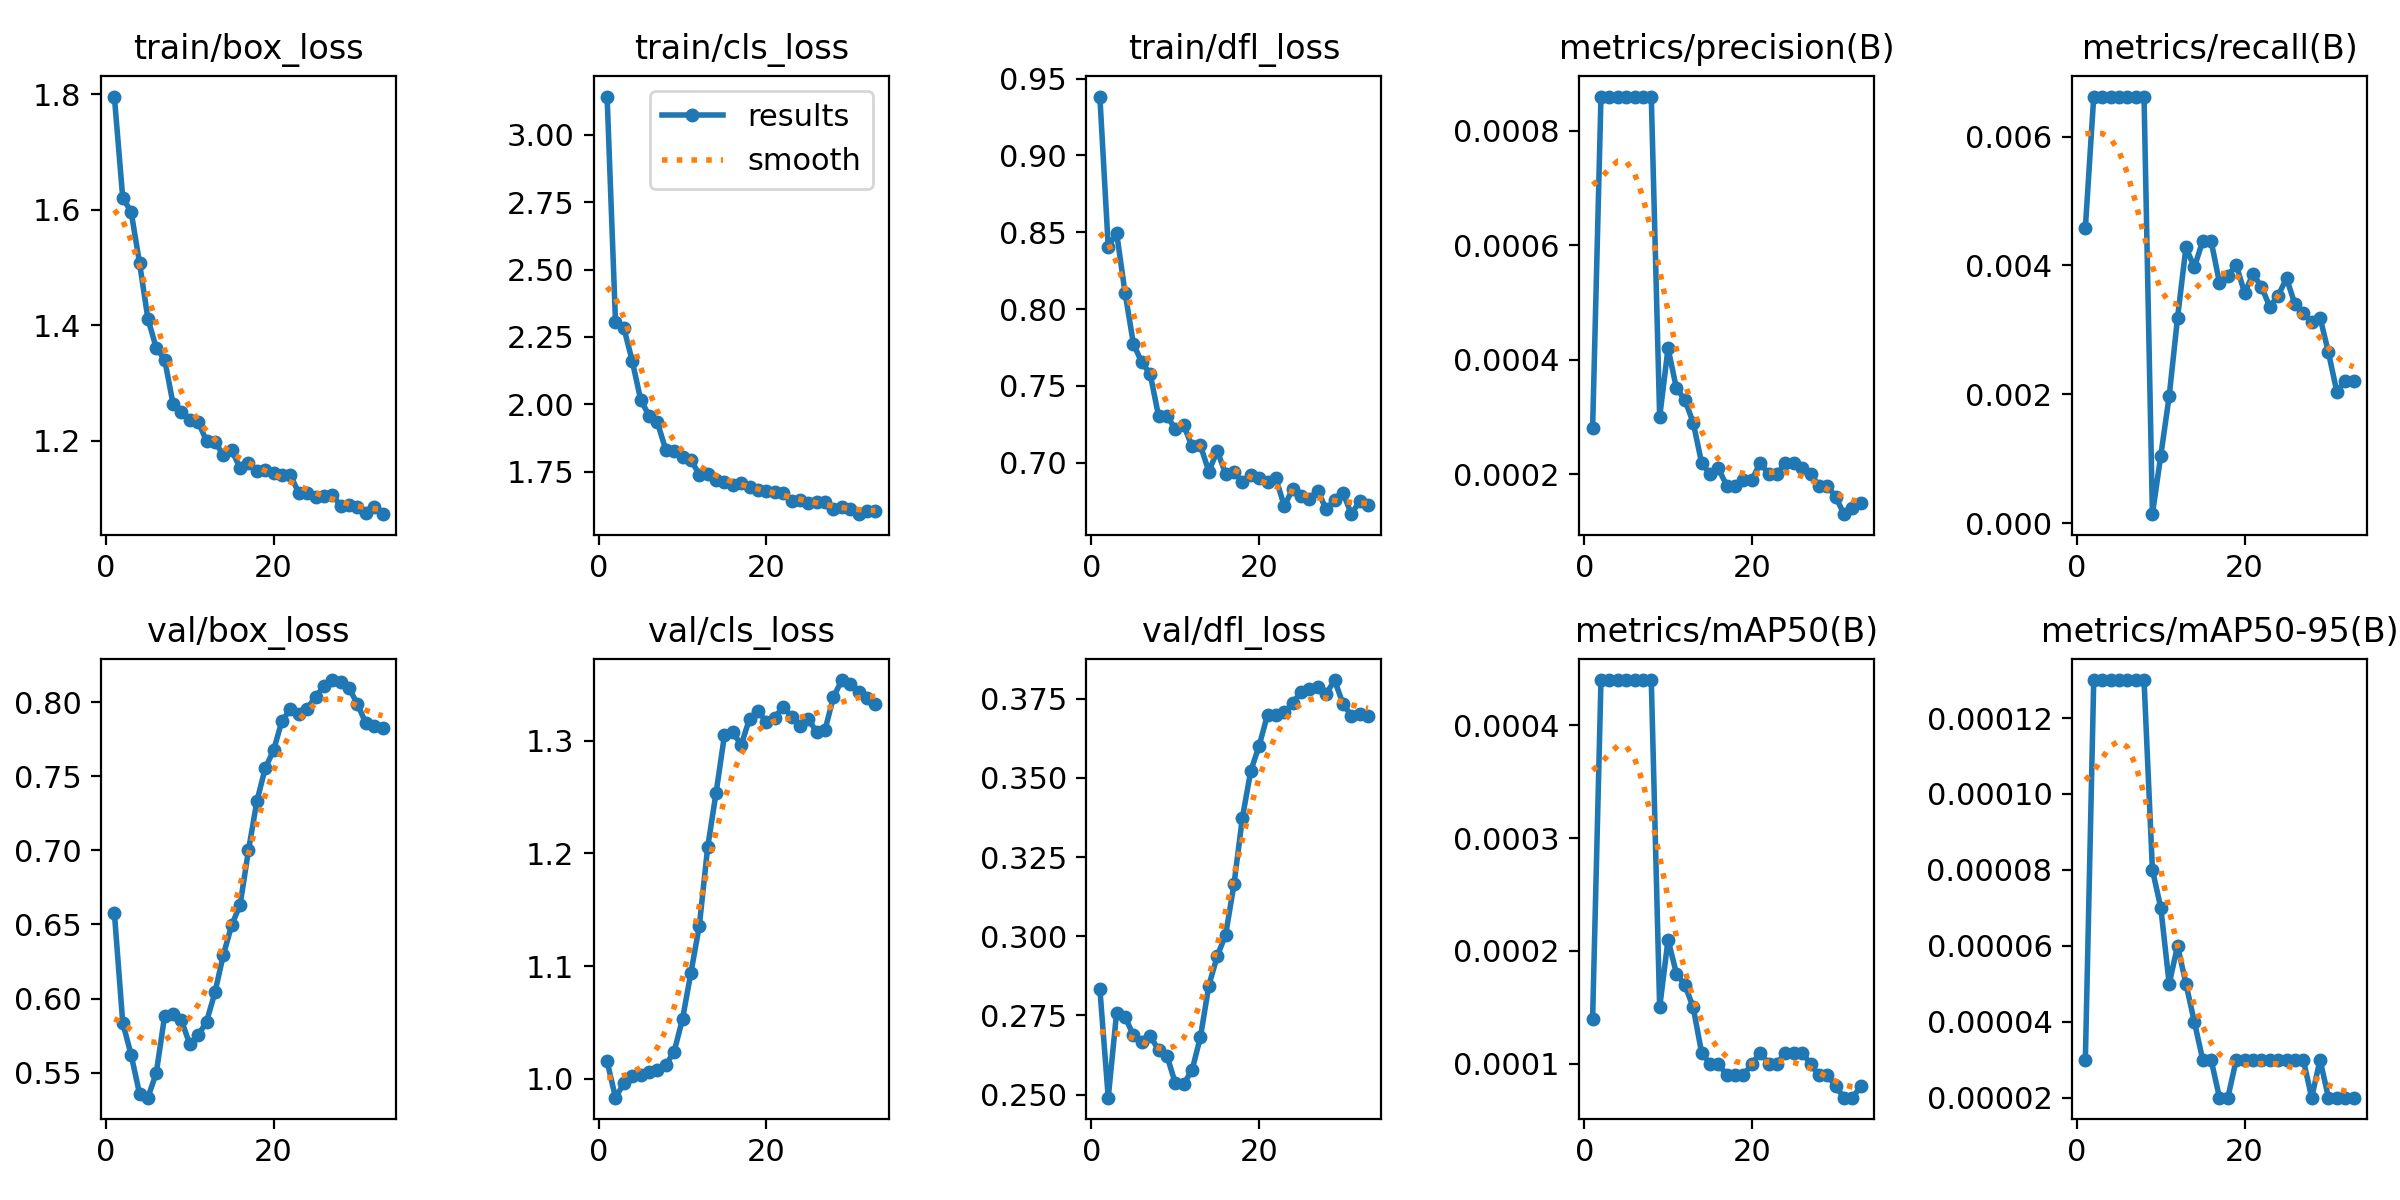
\includegraphics[width=0.8\textwidth]{images/results/bgsub_timeoffset1_results.png}
    \caption{Results of the model training with background subtraction and time offset 1}
    \label{fig:results_bgsub_timeoffset1}
\end{figure}

% TODO results of background subtraction + time offset 1
Because the frames in the video data was just combined with one extra frame to visualize movement in pictures the results of the background subtraction + time offset 1 model are similar to the background subtraction model with almost the same results. So the time offset had no effect on the model.

% HSV
The next results are from the training with the HSV data. The HSV data was created by converting the RGB data to the HSV color space. The results of this training are shown in Table~\ref{fig:results_hsv}.

\begin{figure}[htbp] 
    \centering
    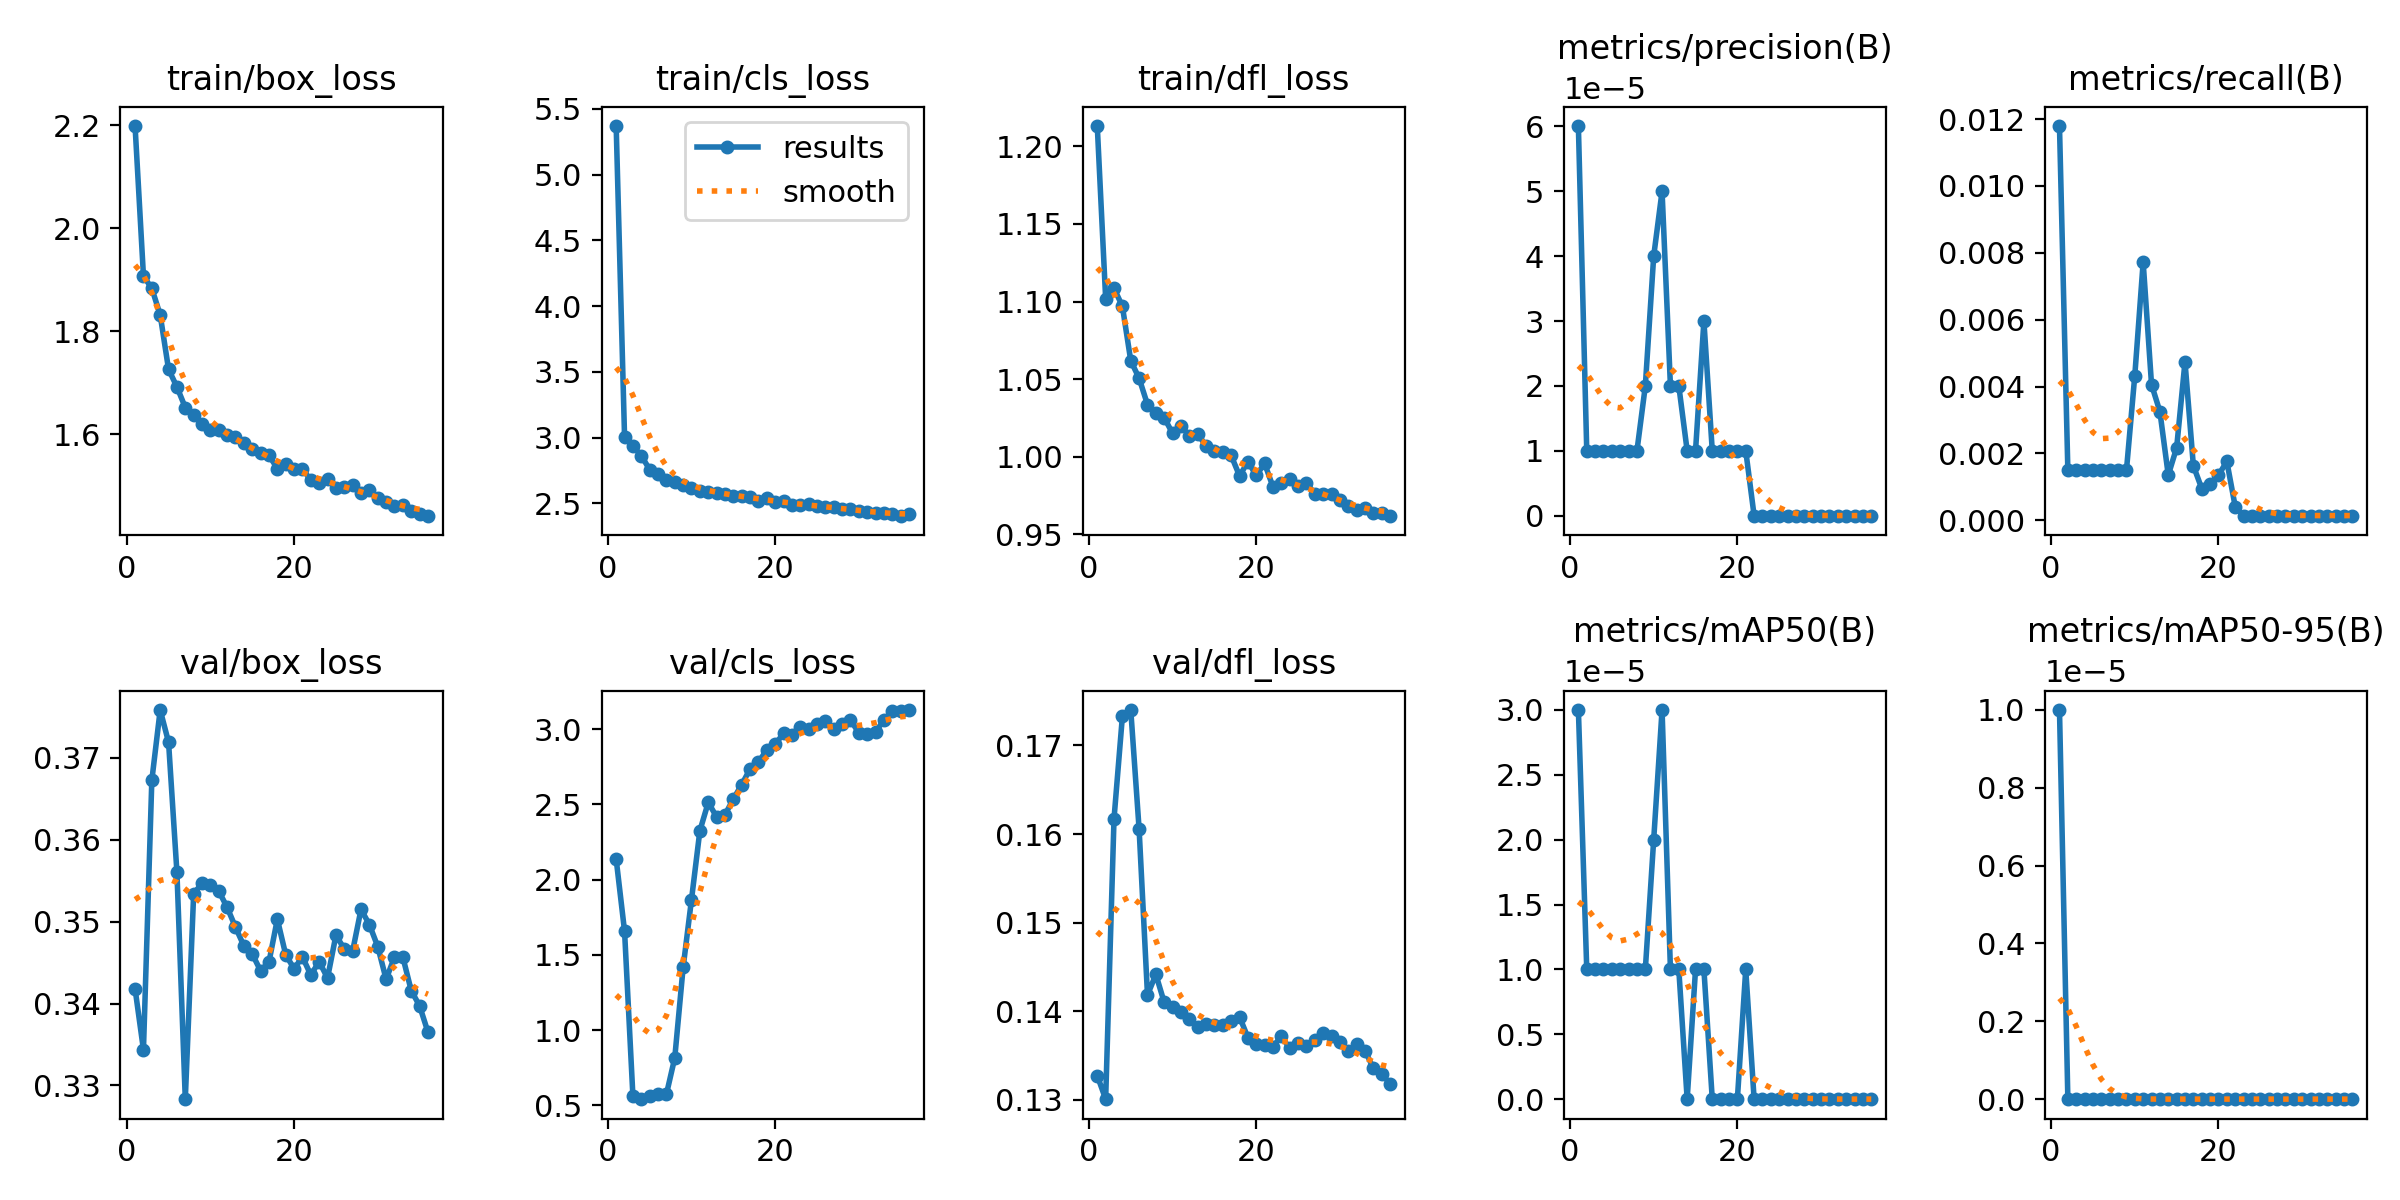
\includegraphics[width=0.8\textwidth]{images/results/hsv_results.png}
    \caption{Results of the model training with HSV data}
    \label{fig:results_hsv}
\end{figure}

% results of hsv
The precision and recall values of the HSV training are very low. They are not going up steadily as they should and even go near zero in the later epochs. Thats a really unnormal progression. The box loss is indeed going down steadily which is a good sign. These results show that the model is not able to detect the insects in the HSV data.

% HSV + background subtraction
The HSV data was then combined with the background subtraction method. The results of this training are shown in Table~\ref{fig:results_hsv_bgsub}.

\begin{figure}[htbp] 
    \centering
    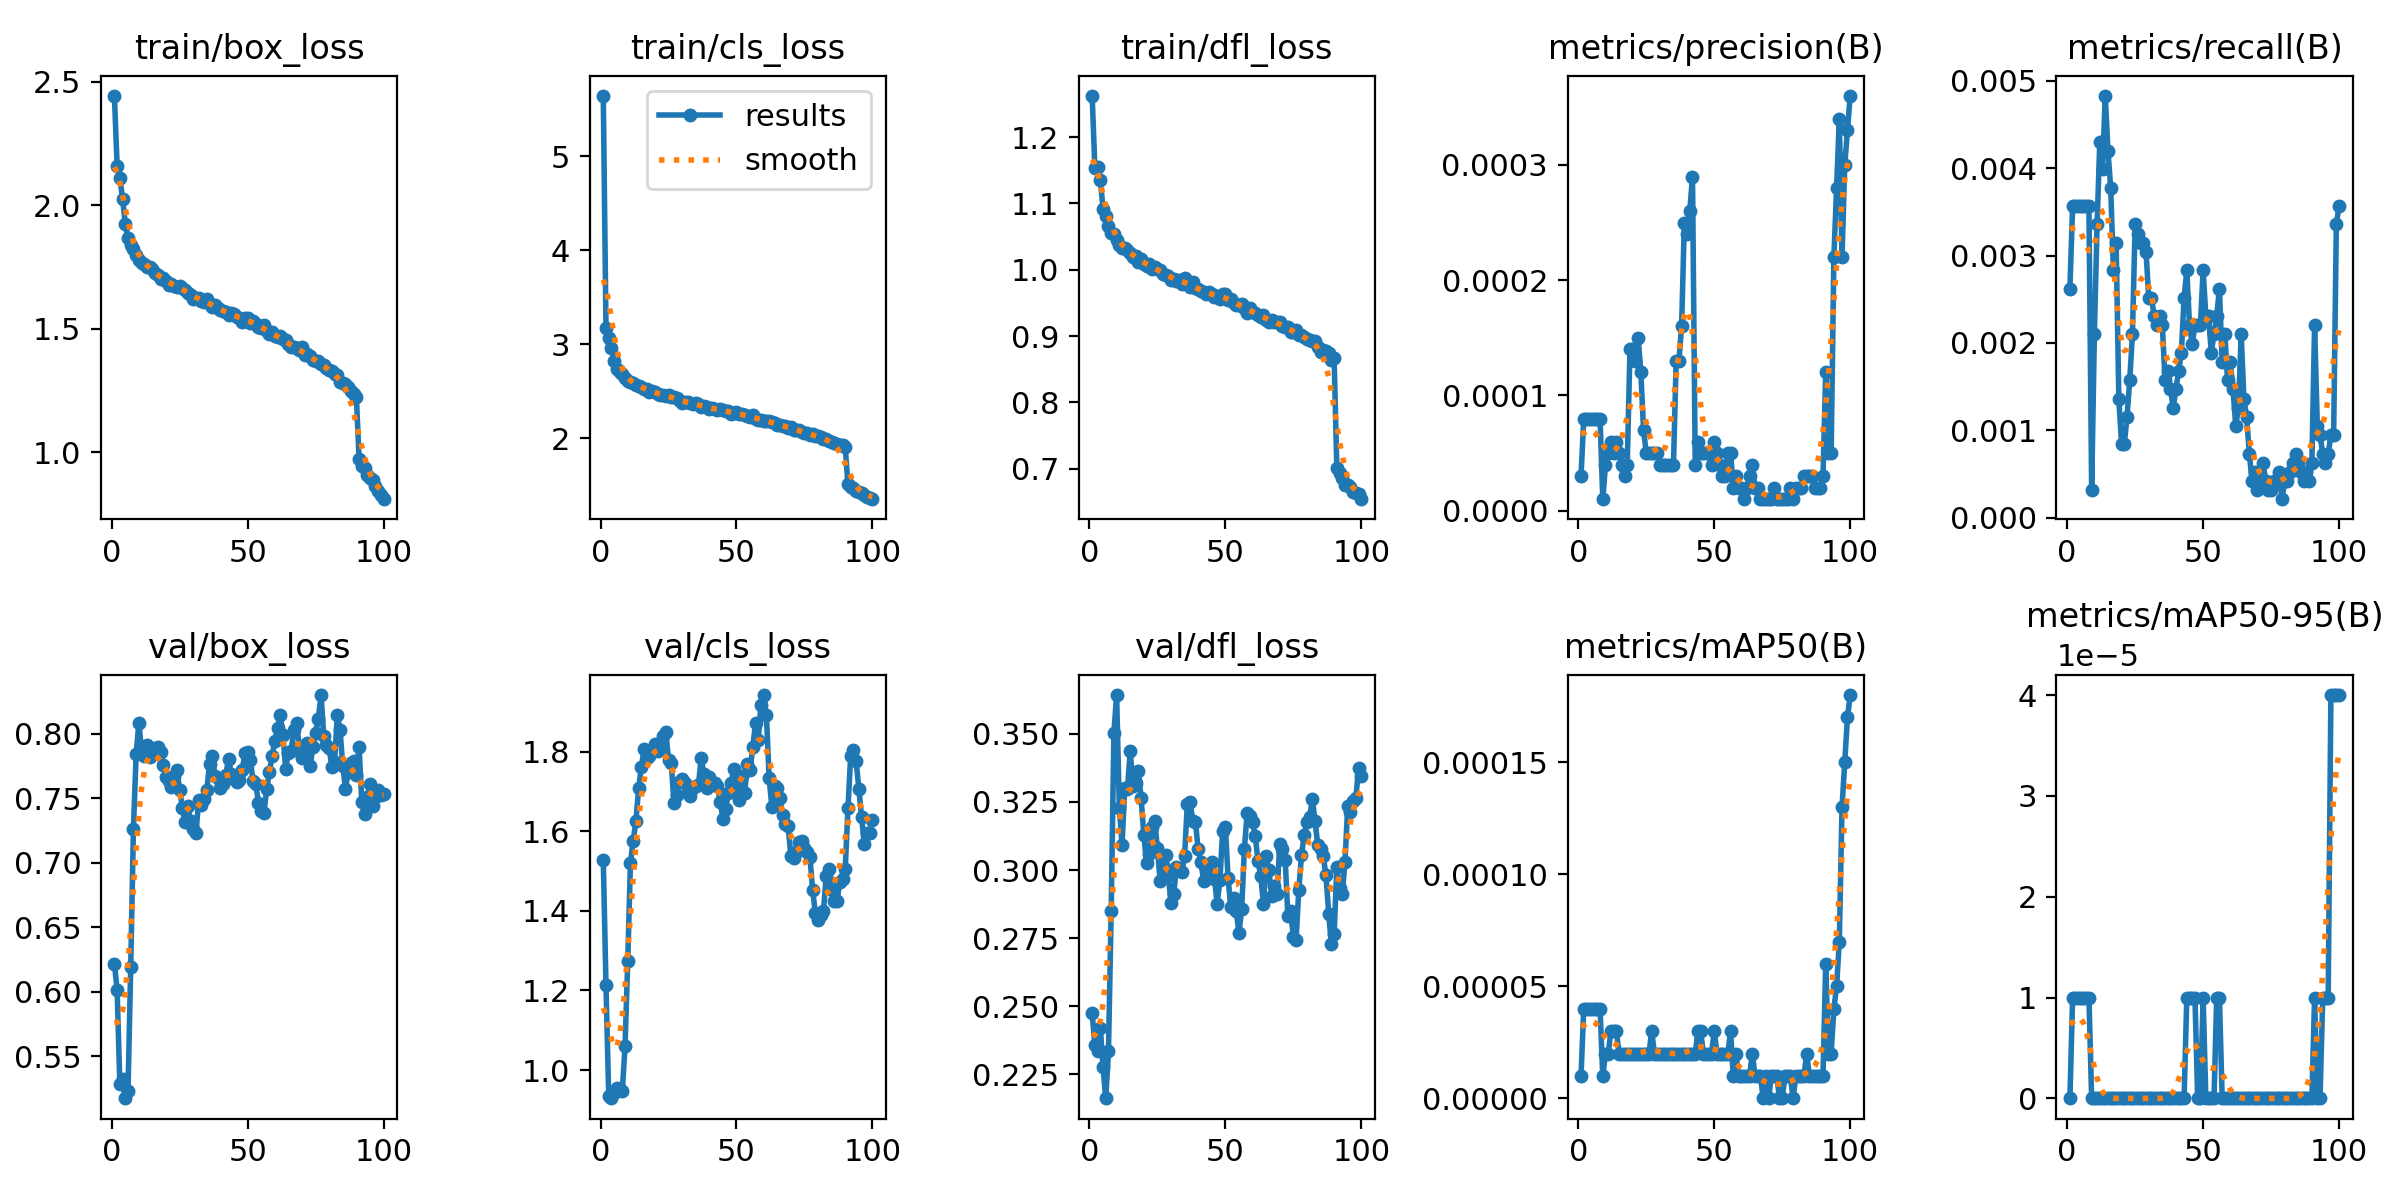
\includegraphics[width=0.8\textwidth]{images/results/hsv_bgsub_results.png}
    \caption{Results of the model training with HSV data and background subtraction}
    \label{fig:results_hsv_bgsub}
\end{figure}

% results of hsv + background subtraction
The results of the model trained with the HSV data and background subtraction is based on the same data as the HSV model. With the background subtraction added the model should perform better than the original HSV model. Firstly the precision and recall values are higher than the original HSV model but still towards zero. Because the precision and recall values are looking not normal the model is not able to detect the insects in the HSV data with the background subtraction.
